\documentclass[10pt,a4paper,draft]{scrartcl}
\usepackage[utf8]{inputenc}

% Page geometry
\usepackage[a4paper, total={15cm,24cm}]{geometry}

% Symbols
\usepackage{amsmath}
\usepackage{amsfonts}
\usepackage{amssymb}

% Graphics
\usepackage{graphicx}
\usepackage{tikz}
\usepackage{tikz-3dplot}

% Language localization
\usepackage[english]{babel}

% Improves float behavior (e.g. enables [H]) and puts captions on top
\usepackage{float}
\floatstyle{plaintop}

% Includes todo-notes (only visible in draft mode)
\usepackage[obeyDraft]{todonotes}

% Makes caption identifiers (i.e. Figure X:) bold
\usepackage[labelfont=bf]{caption}

% Gives \ref and \cite hyperlinks to what they refer to
\usepackage[hidelinks]{hyperref}

% Enables \begin{comment} comments
\usepackage{comment}

% Bold math style, useful for vectors
\usepackage{bm}

\author{Niklas Wingren}
\title{Literature Review}
\subtitle{Summary of activity}

\begin{document}
	
	\maketitle
	
	\section{Introduction}
	This document presents my work during the literature review.
	
	\section{Subjects}
	Before beginning to search for information, some areas of interest were identified. These are listed below:
	
	\begin{itemize}
		\item Non-destructive testing
		\item Micro/mm-wave imaging
		\item Acousto-optics
		\item Acousto-electromagnetism
		\item Aerospace composites
		\item Medical applications of acoustics/microwaves
	\end{itemize}
	
	\begin{comment}
	\subsection{Acousto-electromagnetism}
	What is meant with the term "acousto-electromagnetism" is interaction between acoustics and electromagnetics in a more general sense than what is done in acousto-optics. The primary thought was that this would include phenomena which would occur at lower than optical frequencies (for example at mm-waves).
	
	Much work has been done at the University of Minnesota Radiation Lab when it comes to an electromagnetic view of the interaction \cite{Lawrence2001}\cite{Sarabandi2003}\cite{Buerkle2007}\cite{Buerkle2008}\cite{Buerkle2009}. The mechanism of interaction is based on both density variation and boundary perturbation of a target \cite{Buerkle2007}. The approach is very much based on radar since they consider electromagnetic detection of a discrete target, and acoustic waves are used to better illuminate said target. Analytic solutions exist for dielectric \cite{Lawrence2001} and metallic \cite{Sarabandi2003} infinite cylinders. There are also numeric simulations using the same approach, but for more complex targets \cite{Buerkle2008}\cite{Buerkle2009}.
	\end{comment}
	
	\section{Identified mechanisms}
	In the literature a number of mechanisms have been presented for interaction between acoustics and electromagnetics.
	
	\subsection{Boundary perturbation of target}
	This mechanism is based on a discrete target under acoustic resonance. The resonance of the target leads to vibration, which is seen as a time-dependent boundary perturbation \cite{Buerkle2007}. Vibration causes a micro-Doppler shift in scattered electromagnetic waves, which corresponds to frequency modulation of the returned signal by the frequency of vibration \cite{Chen2006}. For a stationary target this corresponds to a signal with a strong frequency component at $f_c$ and weaker sidebands at $f_c \pm n f_v$ where $n=1$ are the strongest (carrier frequency $f_c$, variation frequency $f_v$, positive integers $n$). The amplitudes of the spectral lines are given by Bessel functions $J_n(B)$, where $B \sim (4\pi/\lambda)D_v$ \cite{Chen2006}. $D_v$ is the amplitude of vibration which is usually small (on the order of $\mu$m) \cite{Buerkle2007}\cite{Top2014}. For small values of $B$ the central component will dominate, and the first Doppler component will be much more prominent than the others. Therefore it makes sense that this first component is the one considered in the literature \cite{Buerkle2007}.
	
	\subsection{Localized harmonic motion}
	This mechanism is similar to boundary perturbation in that it is based on scattering from harmonic motion. The difference is that harmonic motion is introduced in a bulk material instead of a resonating discrete target. The mechanism has been utilized in the medical method of vibro-acoustography and harmonic motion imaging \cite{Wang2018}. Both techniques use amplitude modulated ultrasound to produce a time-harmonic acoustic radiation force in a localized region of a sample. This force then generates time-harmonic displacement, or vibration. In the acoustic methods the vibrating region emits acoustic waves which can be detected \cite{Fatemi1998}\cite{Konofagou2003}.
	
	An electromagnetic wave incident towards the vibrating region will scatter with a frequency shift which corresponds to the frequency of vibration \cite{Top2014}. This is very similar to the boundary perturbation mechanism described before.
	
	One detail omitted before is the two methods of generating radiation force locally. The first method uses amplitude modulated focused ultrasound with its focus on the region of interest \cite{Top2016}. Since amplitude modulated ultrasound exists throughout the beam a force is generated in that entire region. However, the intensity is much higher in the focus so the force is stronger there. The second method instead uses two single-frequency ultrasonic beams which intersect at the region of interest. The frequencies of the two beams differ by a small amount $\Delta \omega$. Superposition at the intersection will then generate localized amplitude modulation by the difference frequency $\Delta \omega$ \cite{Fatemi1998}.
	
	\subsection{Density variation in material}
	
	\subsubsection{Optics-based theory}
	This mechanism is the one used in the theory of acousto-optics \cite{Saleh2007}\cite{Korpel1981}. The main idea is that there is a relation between the density of a material and its index of refraction. Since an acoustic wave consists of periodic compression and rarefaction in a medium, a consequence is that the index of refraction varies with the same period \cite{Saleh2007}. Due to Fresnel reflection, this periodic structure of varying index of refraction acts as a Bragg reflector scattering incident light. The Bragg condition determines the angle of incidence $\theta_B$ required for the light
	\begin{equation*}
		\sin{\theta_B} = \frac{\lambda}{2\Lambda}
	\end{equation*}
	where $\lambda$ is the light wavelength and $\Lambda$ is the acoustic wavelength \cite{Saleh2007}.
	
	There is nothing in the basic theory suggesting that optical frequencies are required for this interaction. At microwave frequencies premittivity is more common to use than index of refraction, but they are related and the principle is the same. An application which uses this principle and has been used for many years is the radio acoustic sounding system \cite{Buerkle2007}. Additionally, though not using the exact Bragg formulation for modeling interaction, some authors have explored other ways of using density variation for microwave frequencies \cite{Lawrence2001}\cite{Merkel2006}. It has been stated, however, that this interaction is very small and resonance is often required (giving rise to boundary perturbation) \cite{Buerkle2007}. This can be understood by looking at the acousto-optic theory. The Bragg condition gives the angle for peak reflectance against the acoustic wave. When considering strength of the interaction, though, an actual value for the reflectance is of interest. This can be found as
%	\begin{equation*}
%		\mathcal{R} = \frac{\pi^2}{2\lambda_0^2} \left( \frac{L}{\sin{\theta}} \right) ^2 \mathcal{M}I_s
%	\end{equation*}
%	where $\lambda_0$ is vacuum light wavelength, $L/\sin{\theta}$ is the oblique distance of light penetration (approximately), $\mathcal{M}$ is a material parameter and $I_s$ is the acoustic intensity \cite{Saleh2007}. Alternatively, the Bragg condition can be used for the equation
	\begin{equation*}
		\mathcal{R} = 2\pi^2n^2 \frac{L^2 \Lambda^2}{\lambda_0^4} \mathcal{M}I_s
	\end{equation*}
	where $n$ is the unperturbed index of refraction, $L$ is the distance of overlap between light and acoustic waves in the acoustic wave direction, $\Lambda$ is the acoustic wavelength, $\lambda_0$ is the vacuum light wavelength, $\mathcal{M}$ is a material parameter and $I_s$ is the acoustic intensity \cite{Saleh2007}. For intense acoustic waves a correction is necessary, giving $\mathcal{R}_e = \sin{^2\sqrt{\mathcal{R}}}$ \cite{Saleh2007}.
	
	The interesting part when it comes to microwave frequencies, however, is the denominator in the first equation. The factor $1/\lambda_0^4$ might be a reason of concern when moving away from the optical regime. Since the wavelength is much longer for mm-waves there should be a large decrease in reflectance, and if too large the scattered signal could be undetectable. However, some examples for optical wavelengths give $\mathcal{R}_e = 0.192$ \cite{Saleh2007}, which is very large when compared with what can be detected in radar \cite{Richards2012}. There are also other variables such as $L$ and $\Lambda$ which might be changed to give a higher reflectance. If the different parameters can be selected to give a scattered signal above the noise floor is a very interesting question which needs to be investigated.
	
	\subsubsection{Radio Acoustic Sounding}
	This mechanism has not only been used in optics, but also in radio meteorology through the Radio Acoustic Sounding System (RASS) \cite{Buerkle2007}. This indicates that the wavelength dependence described above can be offset by other factors to still give a measurable scattered signal. The system is used for temperature sounding since the speed of sound depends on temperature. The Bragg scattering condition is thus affected by a temperature change \cite{Marshall1972}. The systems are usually designed with electromagnetic and acoustic wave sources approximately co-located \cite{Marshall1972}. This corresponds to an angle $\theta \approx 90^\circ$, which changes the Bragg condition to
	\begin{equation*}
		\Lambda = \frac{\lambda}{2}
	\end{equation*}
	
	\subsection{Displacement of scatterers}
	This is a mechanism presented in the field of ultrasound-optical tomography (UOT). The mechanism is based on dynamic multiple scattering of light, which occurs if many scatterers undergoing Brownian motion are considered \cite{Leutz1995}. If an ultrasonic beam is incident on such a sample the scatterers will move due to both Brownian motion and ultrasound, giving rise to a frequency shift in affected photons \cite{Leutz1995}\cite{Elson2011}. In medical applications, movement of the scatterers due to acoustic waves is very straight-forward: their displacement directly follows the acoustic wave \cite{Leutz1995}. This might well be the case for small scatterers which are then part of the wave, but for larger scatterers it gets more complicated. In that case, acoustic radiation force has to be considered for scatterer movement \cite{Torr1984}.
	
	It is interesting to see if this mechanism holds any relevance when it comes to microwave frequencies. The assumption on which the theory rests is that of dynamic multiple light scattering \cite{Leutz1995}. In the existing mm-wave imaging system there is an assumption of sparse defects being the only scatterers \cite{Helander2017}. This is in complete contrast to the theory of dynamic multiple light scattering, which is based on a large number of moving scatterers \cite{Leutz1995}. Since the basic assumptions of the problem and theory are in such stark contrast, it seems likely that this interaction mechanism holds little relevance to the problem at hand.
	
	\section{Focus of investigations}
	After an initial overview of the different interaction mechanisms a decision had to be made concerning the relevance of said mechanisms. Those deemed interesting enough for the problem at hand would be studied further while the others would not.
	
	The boundary perturbation mechanism is based on acoustic resonance in the target. Proposed NDT methods using this mechanism are based on the entire device under test being in acoustic resonance and using Doppler components to find defects \cite{Buerkle2009}. An issue with this is that the resonance frequencies of complex objects are difficult to know beforehand. A possibility would be to scan the acoustic frequency in order to find a resonance, but with an already time-consuming electromagnetic measurement this might be less desirable. Additionally, the mechanism is very similar to localized harmonic motion with one main difference being that the latter does not require resonance. The boundary perturbation mechanism was therefore decided not to be a focus point in further investigations.
	
	As stated above, the localized harmonic motion mechanism has an advantage over boundary perturbation as it does not require resonance. Since the ultrasonic focus can be moved to any point in the device under test, a method using this mechanism is not nearly as dependent on geometry-specific parameters such as resonance frequency. The interaction strength depends on both acoustic, mechanic and electromagnetic properties which should give contrast enhancement when compared with a method using only one phenomenon \cite{Top2016}. This would allow for detection of deviation from the normal in any modality, which could indicate a defect when used in NDT. The freedom in focus selection together with obvious possibilities for contrast made this mechanism worth investigating further.
	
	The density variation mechanism was found in two distinct frequency ranges: acousto-optics and radio acoustic sounding. Even though they are quite different in detail, they use the same interaction mechanism which in itself makes it an interesting topic. It is an indication of some scaling ability, and the big question was to find scaling laws and apply them to the ranges of the NDT problem.
	
	The scatterer displacement mechanism is based on dynamic multiple scattering of light. As explained earlier, this is not very applicable at microwave frequencies, and especially not for the NDT problem. Therefore, this mechanism was not investigated any further.
	
	To summarize, the mechanisms in focus of further investigations were:
	\begin{itemize}
		\item Density variation in material
		\item Localized harmonic motion
	\end{itemize}
	
	\section{Density variation in material - further investigation}
	
	\subsection{Electromagnetics-based theory}
	Instead of using ray and wave optics to explain the interaction (as in \cite{Saleh2007}) it is possible to use electromagnetism. This comes naturally in the field of radio acoustic sounding due to its frequency range, but is also useful in acousto-optics \cite{Korpel1988}. 
	
	From the perspective of radio acoustic sounding, an equation for the electromagnetic scattering against a dielectric disturbance is given by \cite{Gurvich1987}:
	\begin{equation*}
	E_{sc}(\bm{r},t) = \frac{k^2}{4\pi} \int_{V_{sc}} \frac{e^{ik \left| \bm{r}-\bm{r'} \right| }}{ \left| \bm{r}-\bm{r'} \right| } \varepsilon_s (\bm{r'},t) E_0 (\bm{r'},t) \mathrm{d}^3r'
	\end{equation*}
	where $k$ is the wavenumber, $V_{sc}$ is the scattering volume, $\bm{r}$ is the observation point, $\varepsilon_s$ is the variation in relative permittivity and $E_0$ is the incident electric field. The equation is only valid for scattering with no polarization change since polarization is not considered in the electric field. It is also only valid for single scattering \cite{Gurvich1987}.
	
	A more rigorous derivation of electromagnetic scattering against a dielectric perturbation is presented in \cite{Tatarskii1971}. This was used to derive a more general scattering integral than the one presented above (see \ref{app:scatterint} for derivation). This is shown below
	\begin{equation*}
		\bm{E}_{sc}(\bm{r},t) = \frac{1}{4\pi\varepsilon_r} \int_{V_{sc}} \frac{e^{ik |\bm{r}-\bm{r'}| }}{ |\bm{r}-\bm{r'}|} \left( k^2 \bm{E}_i (\bm{r'},t) \varepsilon_1 (\bm{r'},t) + \nabla (\bm{E}_i (\bm{r'},t) \cdot \nabla \varepsilon_1 (\bm{r'},t)) \right) \mathrm{d}v'
	\end{equation*}
	here the electric field is allowed to have any polarization, which is the cause of the second term in the integral. $\varepsilon_r$ is now the unperturbed relative permittivity, $k$ the unperturbed wavenumber in the material and $\varepsilon_1$ a small perturbation in relative permittivity (defined as $\varepsilon = \varepsilon_0(\varepsilon_r + \varepsilon_1)$).
	
	\subsection{Photoelasticity}
	The primary mechanism behind this interaction is, as stated earlier, a variation of density leading to a change in refractive index (or permittivity). To get a full picture of the interaction, the relationship between acoustic intensity and refractive index must be known. For a one-dimensional, longitudinal sound wave the change in refractive index is given by \cite{Saleh2007}
	\begin{equation*}
	\Delta n (x,t) = -\frac{1}{2} \mathfrak{p} n^3 s(x,t)
	\end{equation*}
	where $\mathfrak{p}$ is the photoelastic constant (also called strain-optic coefficient or elasto-optic coefficient \cite{Korpel1988}), $n$ is the unperturbed refractive index and $s(x,t)$ is the acoustic strain. Singe it is negative, a positive strain decreases the refractive index \cite{Saleh2007}.
	
	It is also possible to write this change depending on the acoustic intensity instead of the actual wave. This is done as \cite{Saleh2007}
	\begin{equation*}
	\Delta n_0 = \sqrt{\frac{1}{2} \mathcal{M} I_s} \quad , \quad
	\mathcal{M} = \frac{\mathfrak{p}^2 n^6}{\rho v_s^3}
	\end{equation*}
	where $I_s$ is the acoustic intensity (W/m$^2$), $\rho$ is the mass density and $v_s$ is the speed of sound. The amplitude is related to the total refractive index as \cite{Saleh2007}
	\begin{equation*}
	n(x,t) = n - \Delta n_0 \cos(\Omega t - qx)
	\end{equation*}
	where $\cos(\Omega t - qx)$ comes from a plane acoustic wave.
	
	The refractive index and relative permittivity are related by $\varepsilon_r = n^2$ in a non-magnetic material. To obtain the change in relative permittivity instead of refractive index
	\begin{equation*}
	\Delta \varepsilon_r(x,t) = \frac{\mathrm{d}\varepsilon_r}{\mathrm{d}n} \Delta n(x,t) = 2n \Delta n(x,t) = -\mathfrak{p} \varepsilon_r^2 s(x,t)
	\end{equation*}
	
	However, the photoelastic constant described above is really a simplification of the mechanism. For a full picture it is important to consider the tensor properties from solid mechanics (for acoustics) and optical anisotropy (for electromagnetism) \cite{Korpel1988}. This gives rise to a photoelastic tensor instead of a simple constant. The relation is then given as \cite{Korpel1988}
	\begin{equation*}
	\Delta \left( \frac{1}{n_i^2} \right) = p_{ij} S_j
	\end{equation*}
	where $S_j$ are strains and $i,j = 1,...,6$. The double indexation of $j$ in both $p$ and $S$ indicates a summation over $j$. This can seem a bit troublesome to use since the LHS is the difference of an inverse quantity. This can be rewritten as shown below
	\begin{align*}
	\alpha &= \frac{1}{n_i^2},\ n_i = \alpha^{-1/2} \\
	\Delta n_i &= \frac{\mathrm{d}n_i}{\mathrm{d}\alpha} \Delta \alpha = -\frac{1}{2} \alpha^{-3/2} \Delta \alpha = -\frac{1}{2} n_i^3 p_{ij} S_j
	\end{align*}
	This is similar to the simple relation, but it now has tensor quantities instead of scalar ones. As before this can also be written as permittivity:
	\begin{equation*}
	\Delta \varepsilon_{r_i} = 2n_i\Delta n_i = -n_i^4 p_{ij} S_j = -\varepsilon_{r_i}^2 p_{ij} S_j
	\end{equation*}
	
	The tensor notation here is a simplified form described by the 1949 IRE standards. The relation to full tensor notation is shown below for refractive indices and strains \cite{Korpel1988}
	\begin{align*}
	n_1 &= n_{11},\ n_2 = n_{22},\ n_3 = n_{33}, \\
	n_4 &= n_{23},\ n_5 = n_{31},\ n_6 = n_{12} \\
	S_1 &= \delta_{11},\ S_2 = \delta_{22},\ S_3 = \delta_{33}, \\
	S_4 &= \delta_{23},\ S_5 = \delta_{31},\ S_6 = \delta_{12}
	\end{align*}
	where $\delta_{kl}$ are the strains in standard tensor notation. It is clear that indices 1-3 are tensile and 4-6 are shear. The photoelastic tensor in standard notation is then clearly of rank 4, being $p_{ijkl}$.
	
	The photoelastic tensor can have up to 36 independent components, but for the simple case of an isotropic solid the tensor simplifies to \cite{Korpel1988}
	\begin{align*}
	p_{11} &= p_{22} = p_{33}, \ p_{12} = p_{21} = p_{13} = p_{23} = p_{32}\\
	p_{44} &= p_{55} = p_{66} = \frac{1}{2} (p_{11} - p_{22}), \ p_{ij} = 0 \text{ for others}
	\end{align*}
	
	The simplest material to consider would be an isotropic solid with isotropic permittivity $\varepsilon_r$. There is then no preferred axis and a coordinate system can be selected arbitrarily. A longitudinal acoustic wave is defined by \begin{equation*}
	S_1(x_1,t) = \delta_{11}(x_1,t) = S_0 \cos(\Omega t - qx_1)
	\end{equation*}
	It is propagating in the $x_1$ direction and is thus a strain $S_1$, and all other strains are assumed to be zero. The relation $\Delta \varepsilon_{r_i} = -\varepsilon_{r_i}^2 p_{ij} S_j$ together with the photoelastic tensor for isotropic solids then gives
	\begin{align*}
	\varepsilon_{r_1} &= -\varepsilon_r^2 p_{11} S_0 \cos(\Omega t - qx_1) \\
	\varepsilon_{r_2} &= \varepsilon_{r_3} = -\varepsilon_r^2 p_{12} S_0 \cos(\Omega t - qx_1)
	\end{align*}
	It is clear that the permittivity now has an axis $x_1$ where it has another value than in $x_2$ and $x_3$. So even for a material which is nominally completely isotropic, a preferred axis arises for the permittivity! This type of anisotropy is called birefringence in optics, and in this case it is caused by dipoles aligning themselves parallel to the strain \cite{Korpel1988}. Practically, the effect of this is that the interaction strength of this mechanism depends on the EM polarization with respect to the acoustic wave polarization. In longitudinal acoustic waves the polarization and propagation direction coincide, which makes analysis easier.
	
	Another starting point for the interaction is the Lorentz-Lorenz relation, which leads to the equations \cite{Korpel1988}
	\begin{align*}
	\Delta n &= C' s \\
	C' &= \left[ \frac{(n^2-1)(n^2+2)}{6n} \right](1-\Lambda_0) \\
	\Lambda_0 &= -\left( \frac{\rho}{\alpha} \right) \frac{\mathrm{d} \alpha}{\mathrm{d} \rho}
	\end{align*}
	where $\rho$ is the density and $\alpha$ is the molecular polarizability. Here the anisotropic effects are contained in the parameter $\Lambda_0$ \cite{Korpel1988}. If anisotropy should be considered, the tensor model is probably better to use, but if $\Lambda_0$ is neglected a simplified model is obtained. This type of model is usually accurate for liquids, but many solids do not have this behavior \cite{Korpel1988}. Nevertheless, the simplified relation can be written for permittivity (using $\varepsilon_r = n^2$ and $\Delta \varepsilon_r = 2n \Delta n$) as
	\begin{equation*}
	\Delta \varepsilon_r = \frac{1}{3} (\varepsilon_r - 1)(\varepsilon_r + 2) s
	\end{equation*}
	This can be compared with the previous relation $\Delta \varepsilon_r = -\mathfrak{p}\varepsilon_r^2 s$ to obtain an equivalent photoelasticity
	\begin{equation*}
	\mathfrak{p} = -\frac{(\varepsilon_r - 1)(\varepsilon_r + 2)}{3\varepsilon_r^2}
	\end{equation*}
	This can then be used in all equations derived with $\mathfrak{p}$ relating permittivity and strain. However, it should be noted that this model is extremely simplistic and will probably give faulty results in many cases.
	
	\todo[inline]{Shear waves? They do not cause density variation, but still cause photoelastic interaction. Maybe this entire mechanism should be called photoelastic interaction?}
	
	\subsection{Radar equation}
	If a scalar photoelastic relationship is assumed, the scattering integral can be calculated for a simple geometry. This is done in \ref{app:radareq}, but the results are presented here. The geometry of the problem is shown in figure \ref{fig:radareq-geom-main}. This shows a Cartesian coordinate system, but in the following equations this is transformed into a spherical coordinate system. The reason for this is that a Cartesian system is more suitable to the problem definition and integral calculation, while a spherical system is more suitable to writing the results as a radar equation.
	\begin{figure}[h]
		\centering
		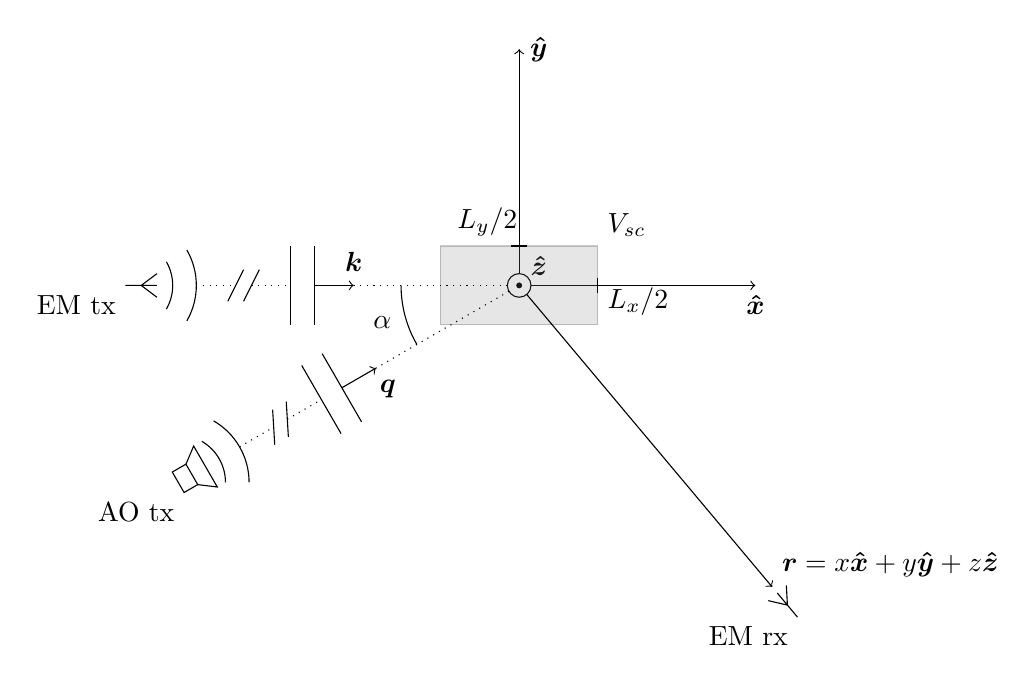
\begin{tikzpicture}
			% Draw coordinate axes
			\draw (0,0) circle(0.15);
			\filldraw[black] circle(0.03);
			\draw[->] (0.15,0) -- (3,0);
			\draw[->] (0,.150) -- (0,3);
			\draw (3,-0.25) node{$\bm{\hat{x}}$} (0.25,3) node{$\bm{\hat{y}}$} (0.25,0.25) node{$\bm{\hat{z}}$};
			
			% Draw scattering cube (or rectangle in this case)
			\draw[fill=gray,opacity=0.2] (-1,-0.5) rectangle(1,0.5);
			\draw (1,-0.1) -- (1,0.1) node[anchor= north west]{$L_x/2$} (-0.1,0.5) -- (0.1,0.5) node[anchor= south east]{$L_y/2$} (1,0.5) node[anchor=south west]{$V_{sc}$};
			
			% Draw EM tx and spherical waves
			\draw[shift = {(-5,0)}] (0,0) node[anchor=north east]{EM tx} -- (0.4,0) (0.2,0) -- (0.4,0.15)
			(0.2,0) -- (0.4,-0.15);
			\draw[shift = {(-5,0)}] ([shift={(-30:0.6)}] 0,0) arc(-30:30:0.6) ([shift={(-30:0.9)}] 0,0) arc(-30:30:0.9);
			
			% Draw EM "long distance" lines
			\draw[shift = {(-4.1,0)},dotted] (0,0) -- (0.5,0) (0.7,0) -- (1.2,0);
			\draw[shift = {(-4.1,0)}] (0.4,-0.2) -- (0.6,0.2) (0.6,-0.2) -- (0.8,0.2);
			
			% Draw EM plane waves
			\draw[shift = {(-2.9,0)}] (0,-0.5) -- (0,0.5) (0.3,-0.5) -- (0.3,0.5);
			\draw[shift = {(-2.6,0)}, ->] (0,0) -- (0.5,0);
			\draw[shift = {(-2.6,0)}] (0.5,0.3) node{$\bm{k}$};
			\draw[dotted] (-0.15,0) -- (-2.1,0);
			
			% Draw AO tx and spherical waves
			\draw[shift = {(210:5)}, rotate = 30] (0,-0.15) node[anchor=north east]{AO tx} rectangle (0.2,0.15) -- (0.4,0.3) -- (0.4,-0.3) -- (0.2,-0.15);
			\draw[shift = {(210:5)}, rotate = 30] ([shift={(-30:0.6)}] 0,0) arc(-30:30:0.6) ([shift={(-30:0.9)}] 0,0) arc(-30:30:0.9);
			
			% Draw AO "long distance" lines
			\draw[shift = {(210:4.1)}, rotate = 30,dotted] (0,0) -- (0.5,0) (0.7,0) -- (1.2,0);
			\draw[shift = {(210:4.1)}, rotate = 30] (0.4,-0.2) -- (0.6,0.2) (0.6,-0.2) -- (0.8,0.2);
			
			% Draw AO plane waves
			\draw[shift = {(210:2.9)}, rotate = 30] (0,-0.5) -- (0,0.5) (0.3,-0.5) -- (0.3,0.5);
			\draw[shift = {(210:2.6)}, rotate = 30, ->] (0,0) -- (0.5,0);
			\draw[shift = {(210:2.6)}, rotate = 30] (0.5,-0.3) node{$\bm{q}$};
			\draw[rotate = 30, dotted] (-0.15,0) -- (-2.1,0);
			
			% Draw angle alpha
			\draw ([shift={(180:1.5)}] 0,0) arc(180:210:1.5) (195:1.8) node{$\alpha$};
			
			% Draw line towards receiver
			\draw[->] (310:0.15) -- (310:5) node[anchor=south west]{$\bm{r} = x\bm{\hat{x}} + y\bm{\hat{y}} + z\bm{\hat{z}}$};
			
			% Draw EM rx
			\draw[shift = {(310:5.5)}, rotate = 130] (0,0) node[anchor=north east]{EM rx} -- (0.4,0) (0.2,0) -- (0.4,0.15) (0.2,0) -- (0.4,-0.15);
		\end{tikzpicture}
		\caption{\label{fig:radareq-geom-main} Geometry for the scattering problem.}
	\end{figure}

	An equation for the received power is written as
	\begin{equation*}
	P_R^\pm = \frac{P_T R_T G_R \lambda_R^2 \sigma^\pm (\theta,\phi)}{(4\pi)^3 R_T^2 R_R^2}
	\end{equation*}
	with the radar cross-section given by
	\begin{equation*}
	\sigma^\pm (\theta, \phi) = \frac{\varepsilon_r^2 k^4}{16\pi} \mathfrak{p}^2 S_0^2 L_x^2 L_y^2 L_z^2 \Phi^\pm (\theta,\pi)^2
	\end{equation*}
	and the angular dependence is contained in $\Phi^\pm$ which is given by
	\begin{multline*}
	\Phi^\pm(\theta,\phi) = \text{sinc} \left( \frac{L_x}{2\pi} \left( k - k\sin{\theta}\cos{\phi} \pm q\cos{\alpha} \right) \right) 
	\cdot \text{sinc} \left( \frac{L_y}{2\pi} \left( -k\sin{\theta}\sin{\phi} \pm q\sin{\alpha} \right) \right) \\
	\cdot \text{sinc} \left( -\frac{L_z}{2\pi} k\cos{\theta} \right)
	\end{multline*}
	The received power has two frequency components: $\omega + \Omega$ and $\omega - \Omega$. The $\pm$-sign in the equations is used to differentiate between the two components. The equations strictly holds only for frequency components separated in space. If the two components overlap, the total received power will be comprised of the power for both components as well as a time-dependent mixing term. This will behave as an amplitude modulated signal. However, as will be shown there is usually no overlap between the two components. To see this, the function for angular angular dependence, $\Phi$ is considered. Only here in the equation for received power do the two components differ. This function varies between 0 and 1 and depends only on the geometry of the problem. The $\theta$, $\phi$ and $\alpha$ where this function is maximized gives the geometry at which maximum scattering is produced. The maximum is derived in \ref{app:braggmax} and is described by the equations
	\begin{align*}
		\theta &= \pi/2 \\
		\cos{\alpha} = \mp \frac{q}{2k} &= \mp \frac{\lambda}{2\Lambda} \\
		\tan{\frac{\phi}{2}} = \pm \sqrt{\frac{q^2}{4k^2-q^2}} &= \pm \sqrt{\frac{\lambda^2}{4\Lambda^2-\lambda^2}}
	\end{align*}
	The equation for $\alpha$ shows what the angle between the incident electromagnetic and acoustic waves should be, and the equations for $\theta$ and $\phi$ show where the receiver should be placed. The first equation shows clearly that the interaction occurs in a plane since $\theta = \pi/2$ is the $xy$-plane defined by the incident waves. The second equation corresponds directly to the Bragg condition presented in acousto-optic theory (see \ref{app:braggmax}). The third equation is not present in acousto-optics since it is implied that an incident light wave is reflected corresponding to optical laws (incident angle equals reflected angle) \cite{Saleh2007}. The equation is nevertheless in agreement with acousto-optics if suitable variable substitutions are used (see \ref{app:braggmax}).
	
	If the equations for maximization of $\Phi$ are studied, the angles where there is overlap between the two components can be found. For overlap to happen, it must hold that $\theta = \pi/2$, $\cos{\alpha} = -\cos{\alpha}$ and $\tan{\frac{\phi}{2}} = -\tan{\frac{\phi}{2}}$. First, $\alpha$ is considered. The angle is defined between 0 and $\pi$, and in this range $\cos{\alpha} = -\cos{\alpha}$ holds only for $\alpha = \pi/2$. This gives $\lambda/2\Lambda = 0$. If this is inserted in the equation for $\phi$, $\tan{\frac{\phi}{2}} = 0$ is obtained, which gives $\phi = 0$. The only time overlap is a concern is therefore when $\lambda/\Lambda \rightarrow 0$. However, this is not very practical since the acoustic wavelength must be very large (assuming a limited range of possible electromagnetic wavelengths) and the scattering angle approaches zero.
	
	For practical applications, it is usually more reasonable to use signal-to-noise ratio (SNR) than received power. The radar equation using this quantity is instead written as
	\begin{equation*}
	\textit{SNR}^\pm_N = \frac{P_T R_T G_R \lambda_R^2 \sigma^\pm (\theta,\phi)}{(4\pi)^3 R_T^2 R_R^2 kT_0 B \cdot \mathit{NR}} N
	\end{equation*}
	This also includes a coherent integration of $N$ samples to improve the SNR.
	
	\subsubsection{Numerical example}
	
	\appendix
	
	\section{Miscellaneous/appendix}
	This section is for stuff I don't know where to put yet or stuff not fitting elsewhere.
	
%	\subsection{Derivation of Gurvich scattering equation}
%	Here follows a derivation of equation (2) in \cite{Gurvich1987} from equation (15) in the same. Equation 15 is
%	\begin{equation*}
%		E_{sc} (\bm{r},t) = -\frac{1}{4\pi c^2} \frac{\partial^2}{\partial t^2} \int_{V_{sc}}
%		\varepsilon_s\left( \bm{r}, t - \frac{\left|\bm{r}-\bm{r'}\right|}{c} \right)\\
%		\cdot E_0 \left( \bm{r}, t - \frac{\left|\bm{r}-\bm{r'}\right|}{c} \right)
%		\frac{\mathrm{d}^3r'}{\left|\bm{r}-\bm{r'}\right|}
%	\end{equation*}
%	A time-dependence is assumed as
%	\begin{align*}
%		&\varepsilon_s(\bm{r}, t) = \varepsilon_s(\bm{r}) e^{-i\Omega_0 t} \\
%		&E_0(\bm{r},t) = E_0(\bm{r}) e^{-i\omega_0 t}
%	\end{align*}
%	The original equation can now be rewritten as
%	\begin{equation*}
%	E_{sc} (\bm{r},t) = -\frac{1}{4\pi c^2}
%	\frac{\partial^2}{\partial t^2} \left( e^{-i(\omega_0 + \Omega_0)t} \right) \\
%	\cdot \int_{V_{sc}} e^{i\frac{\omega_0 + \Omega_0}{c} |\bm{r}-\bm{r'}|}
%	\varepsilon_s(\bm{r}) E_0 (\bm{r})
%	\frac{\mathrm{d}^3r'}{\left|\bm{r}-\bm{r'}\right|}
%	\end{equation*}
%	Differentiation and combination of the fields and time-dependencies again gives
%	\begin{equation*}
%	E_{sc} (\bm{r},t) = -\frac{(\omega_0 + \Omega_0)^2}{4\pi c^2}
%	\int_{V_{sc}} e^{i\frac{\omega_0 + \Omega_0}{c} |\bm{r}-\bm{r'}|}\\
%	\cdot \varepsilon_s(\bm{r},t) E_0 (\bm{r},t)
%	\frac{\mathrm{d}^3r'}{\left|\bm{r}-\bm{r'}\right|}
%	\end{equation*}
%	If $\omega_0 \gg \Omega_0$ an approximation can be done as $(\omega_0 + \Omega_0)/c \approx k$ where $k$ is the incident wavenumber. This gives
%	\begin{equation*}
%	E_{sc}(\bm{r},t) \approx \frac{k^2}{4\pi} \int_{V_{sc}} \frac{e^{ik \left| \bm{r}-\bm{r'} \right| }}{ \left| \bm{r}-\bm{r'} \right| } \varepsilon_s (\bm{r'},t) E_0 (\bm{r'},t) \mathrm{d}^3r'
%	\end{equation*}
%	which is equation (2) in \cite{Gurvich1987}.
	
	\subsection{Derivation of scattering integral in density variation \label{app:scatterint}}
	Here follows a formal derivation of the scattering of electromagnetic waves against a perturbation in relative permittivity. This is useful in photoelastic interaction since an acoustic wave in that case causes a periodic dielectric perturbation. Most of this derivation is based on a similar derivation by Tatarskii which considers scattering from turbulence in air \cite{Tatarskii1971}.
	
	\subsubsection{General equation for electric field in perturbated dielectric}
	First, Maxwell's equations for a linear, non-magnetic, source-free, isotropic dielectric are presented. Note that the permittivity is not homogeneous.
	\begin{align*}
		&\nabla \times \bm{\mathcal{E}} = -\mu_0 \frac{\partial \bm{\mathcal{H}}}{\partial t} \\
		&\nabla \times \bm{\mathcal{H}} = \frac{\partial (\varepsilon \bm{\mathcal{E}})}{\partial t} \\
		&\nabla \cdot (\varepsilon \bm{\mathcal{E}}) = 0 \\
		&\nabla \cdot \bm{\mathcal{H}} = 0
	\end{align*}
	The script letters are used here to indicate a time dependence as
	\begin{align*}
		&\bm{\mathcal{E}}(\bm{r},t) = \bm{E}(\bm{r},t) \text{e}^{-i\omega t} \\
		&\bm{\mathcal{H}}(\bm{r},t) = \bm{H}(\bm{r},t) \text{e}^{-i\omega t} \\
	\end{align*}
	This is used to remove the e$^{-i\omega t}$ dependence in the equations and only keep "slower" time dependencies. The new equations are
	\begin{align*}
		&\nabla \times \bm{E} = i\omega \mu_0 \bm{H} - \mu_0 \frac{\partial \bm{H}}{\partial t} \\
		&\nabla \times \bm{H} = -i\omega \varepsilon \bm{E} + \mu_0 \frac{\partial (\varepsilon \bm{E})}{\partial t} \\
		&\nabla \cdot (\varepsilon \bm{E}) = 0 \\
		&\nabla \cdot \bm{H} = 0
	\end{align*}
	Now $\nabla \times$ is applied to $\nabla \times \bm{E}$ and it is combined with $\nabla \times \bm{H}$, giving
	\begin{equation*}
		\nabla \times (\nabla \times \bm{E}) = \omega^2 \mu_0 \varepsilon \bm{E} + 2i\omega \mu_0 \frac{\partial (\varepsilon \bm{E})}{\partial t} - \mu_0 \frac{\partial^2 (\varepsilon \bm{E})}{\partial t^2}
	\end{equation*}
	The relation $\nabla \times (\nabla \times \bm{E}) = -\nabla^2\bm{E} + \nabla(\nabla \cdot \bm{E})$ is now used
	\begin{equation*}
		\nabla^2\bm{E} + \omega^2 \mu_0 \varepsilon \bm{E} = \nabla(\nabla \cdot \bm{E}) - 2i\omega \mu_0 \frac{\partial (\varepsilon \bm{E})}{\partial t} + \mu_0 \frac{\partial^2 (\varepsilon \bm{E})}{\partial t^2}
	\end{equation*}
	Gauss' law $\nabla \cdot (\varepsilon \bm{E}) = 0$ is now expanded to $\varepsilon(\nabla \cdot \bm{E}) + (\nabla \varepsilon) \cdot \bm{E} = 0$. This can be rewritten as
	\begin{equation*}
		\nabla \cdot \bm{E} = -\bm{E} \cdot \frac{\nabla \varepsilon}{\varepsilon} = -\bm{E} \cdot \nabla (\ln{\varepsilon})
	\end{equation*}
	Inserting this into the previous equation gives
	\begin{equation*}
		\nabla^2\bm{E} + \omega^2 \mu_0 \varepsilon \bm{E} = -\nabla(\bm{E} \cdot \nabla (\ln{\varepsilon})) - 2i\omega \mu_0 \frac{\partial (\varepsilon \bm{E})}{\partial t} + \mu_0 \frac{\partial^2 (\varepsilon \bm{E})}{\partial t^2}
	\end{equation*}
	Now, the dielectric perturbation is defined as
	\begin{equation*}
	\varepsilon = \varepsilon_0(\varepsilon_r + \varepsilon_1)
	\end{equation*}
	where $\varepsilon_0$ is the permittivity of free space, $\varepsilon_r$ is the unperturbed value for relative permittivity in the material and $\varepsilon_1$ is a small perturbation around $\varepsilon_r$. For $|\varepsilon_1| \ll \varepsilon_r$ $\ln{\varepsilon}$ can be approximated as
	\begin{equation*}
		\ln{\varepsilon} = \ln(\varepsilon_0 \varepsilon_r) + \ln(1 + \frac{\varepsilon_1}{\varepsilon_r}) \approx \ln(\varepsilon_0 \varepsilon_r) + \frac{\varepsilon_1}{\varepsilon_r}
	\end{equation*}
	Since $\ln(\varepsilon_0 \varepsilon_r)$ is constant, the gradient can be written as
	\begin{equation*}
		\nabla(\ln{\varepsilon}) = \nabla \left( \frac{\varepsilon_1}{\varepsilon_r} \right) = \frac{1}{\varepsilon_r} \nabla \varepsilon_1
	\end{equation*}
	This is now inserted in the equation for the electric field together with the definition of the perturbation:
	\begin{equation*}
		\nabla^2\bm{E} + \omega^2 \mu_0 \varepsilon_0 \varepsilon_r \bm{E} = \\
		 -\omega^2 \mu_0 \varepsilon_0 \varepsilon_1 \bm{E} -\frac{1}{\varepsilon_r}\nabla(\bm{E} \cdot \nabla \varepsilon_1) - 2i\omega \mu_0 \frac{\partial (\varepsilon \bm{E})}{\partial t} + \mu_0 \frac{\partial^2 (\varepsilon \bm{E})}{\partial t^2}
	\end{equation*}
	Now $k$ is defined as $k = \omega/c$ where $c$ is the speed of light in the material
	\begin{equation*}
		c = \frac{1}{\sqrt{\mu_0 \varepsilon_0 \varepsilon_r}} = \frac{c_0}{\sqrt{\varepsilon_r}}
	\end{equation*}
	Now the equation for $\bm{E}$ is written as
	\begin{equation*}
	\boxed{
		\nabla^2\bm{E} + k^2 \bm{E} = \\
		-k^2 \frac{\varepsilon_1}{\varepsilon_r} \bm{E} -\frac{1}{\varepsilon_r}\nabla(\bm{E} \cdot \nabla \varepsilon_1) - \frac{2ik}{c\varepsilon_0\varepsilon_r} \frac{\partial (\varepsilon \bm{E})}{\partial t} + \frac{1}{c^2 \varepsilon_0 \varepsilon_r} \frac{\partial^2 (\varepsilon \bm{E})}{\partial t^2}
	}
	\end{equation*}
	
	\subsubsection{Approximating the right hand side}
	To simplify this equation even more, approximations concerning the nature of the perturbation must be done. The dielectric perturbation is thus assumed to have the following behavior:
	\begin{equation*}
		\varepsilon_1 (\bm{r},t) = |\varepsilon_1| \cos(\bm{q} \cdot \bm{r} - \Omega t)
	\end{equation*}
	where $|\varepsilon_1|$ is the amplitude, $q$ is the acoustic wavevector and $\Omega$ is the acoustic frequency. Furthermore, the relations between wavenumbers and wavelengths are introduced as $k = 2\pi/\lambda$ for electromagnetics and $q = |\bm{q}| = 2\pi/\Lambda$ for acoustics.
	
	Now the terms on the right-hand side (RHS) are estimated to see which terms are dominant. The terms are denoted $T_n$ where $n$ begins at 1 and is the order in which they appear at the RHS. Note that these estimations are only to find orders of magnitude. For the first term:
	\begin{equation*}
		T_1 \sim \frac{|\varepsilon_1| |\bm{E}|}{\varepsilon_r \lambda^2}
	\end{equation*}
	For term 2 $\nabla \varepsilon_1 \sim \Lambda^{-1} |\varepsilon_1| \bm{v}$ where $\bm{v}$ is a vector with components $\sim \sin(\bm{q} \cdot \bm{r} - \Omega t)$. Then $\nabla (\bm{\hat{E}} \cdot \bm{v}) \sim \nabla(|\bm{\hat{E}}| \sin(\bm{q} \cdot \bm{r} - \Omega t)) \sim \nabla(|\bm{\hat{E}}|) + \nabla(\sin(\bm{q} \cdot \bm{r} - \Omega t)) \sim \lambda^{-1} + \Lambda^{-1}$. The resulting estimation of the term is then
	\begin{equation*}
		T_2 \sim \frac{|\varepsilon_1| |\bm{E}|}{\varepsilon_r \Lambda} \left( \frac{1}{\Lambda} + \frac{1}{\lambda} \right)
	\end{equation*}
	Term 3 can be expanded using the perturbation definition and the chain rule:
	\begin{equation*}
		T_3 \sim \frac{k}{c\varepsilon_0\varepsilon_r} \frac{\partial (\varepsilon \bm{E})}{\partial t} = \frac{k}{c\varepsilon_0\varepsilon_r} \left( \varepsilon_0\varepsilon_r \frac{\partial \bm{E}}{\partial t} + \varepsilon_0\varepsilon_1 \frac{\partial \bm{E}}{\partial t} + \varepsilon_0\bm{E} \frac{\partial \varepsilon_1}{\partial t}\right)
		\sim \frac{1}{c\lambda} \left( \frac{\partial \bm{E}}{\partial t} + \frac{\varepsilon_1}{\varepsilon_r} \frac{\partial \bm{E}}{\partial t} + \frac{\bm{E}}{\varepsilon_r} \frac{\partial \varepsilon_1}{\partial t} \right)
	\end{equation*}
	The derivatives can be approximated as
	\begin{align*}
		\frac{\partial \varepsilon_1}{\partial t} &\sim |\varepsilon_1|\Omega \sim \frac{|\varepsilon_1| v}{\Lambda} \\
		\frac{\partial \bm{E}}{\partial t} &\sim \bm{E} v \left( \frac{1}{\Lambda} + \frac{1}{\lambda} \right)
	\end{align*}
	where $v$ is the speed of sound in the material. The second equation comes from a similar equation in \cite{Tatarskii1971} which takes into account the Doppler effect and changes in $\varepsilon_1$. These are inserted to give
	\begin{equation*}
		T_3 \sim \frac{1}{c\lambda} \left( |\bm{E}| v \left( \frac{1}{\Lambda} + \frac{1}{\lambda} \right) \left( 1 + \frac{|\varepsilon_1|}{\varepsilon_r} \right) + \frac{|\bm{E}| |\varepsilon_1| v}{\varepsilon_r \Lambda} \right) =
		\frac{|\bm{E}| |\varepsilon_1| v}{c\lambda} \left( \left( 1 + \frac{|\varepsilon_1|}{\varepsilon_r} \right) \left( \frac{1}{\Lambda} + \frac{1}{\lambda} \right) + \frac{|\varepsilon_1|}{\varepsilon_r \Lambda} \right)
	\end{equation*}
	Now, the condition $|\varepsilon_1| \ll \varepsilon_r$, or equivalently, $|\varepsilon_1|/\varepsilon_r \ll 1$ is used to write the the term as
	\begin{equation*}
		T_3 \sim \frac{|\bm{E}| |\varepsilon_1| v}{c\lambda} \left( \frac{1}{\Lambda} + \frac{1}{\lambda} \right)
	\end{equation*}
	Term 3 can now be compared with term 1 and 2 to determine the relative sizes.
	\begin{align*}
		\frac{T_3}{T_1} &= \frac{|\bm{E}| |\varepsilon_1| v}{c\lambda} \left( \frac{1}{\Lambda} + \frac{1}{\lambda} \right)
		\bigg/
		\frac{|\varepsilon_1| |\bm{E}|}{\varepsilon_r \lambda^2} =
		\frac{v}{c} \frac{\varepsilon_r}{|\varepsilon_1|} \left( 1 + \frac{\lambda}{\Lambda} \right) \\
		\frac{T_3}{T_2} &= \frac{|\bm{E}| |\varepsilon_1| v}{c\lambda} \left( \frac{1}{\Lambda} + \frac{1}{\lambda} \right)
		\bigg/
		\frac{|\varepsilon_1| |\bm{E}|}{\varepsilon_r \Lambda} \left( \frac{1}{\Lambda} + \frac{1}{\lambda} \right) =
		\frac{v}{c} \frac{\varepsilon_r}{|\varepsilon_1|} \frac{\Lambda}{\lambda}
	\end{align*}
	Inspection of these fractions reveals that the condition required for $T_3$ to be neglected is
	\begin{equation*}
		\frac{v}{c} \ll \frac{|\varepsilon_1|}{\varepsilon_r}
	\end{equation*}
	This holds for any ratio between $\lambda$ and $\Lambda$. If $\lambda \gg \Lambda$, $T_2$ will dominate $T_3$. If $\Lambda \gg \lambda$, $T_1$ will dominate $T_3$. If $\lambda \sim \Lambda$, both $T_1$ and $T_2$ will dominate $T_3$. The fourth term on the RHS is similar to the third, but contains a factor $(v/c)^2$. Thus, if $T_3$ can be neglected, so can $T_4$.	The simplified equation if the condition $v/c \ll |\varepsilon_1|/\varepsilon_r$ holds is shown below:
	\begin{equation*}
	\boxed{
		\nabla^2\bm{E} + k^2 \bm{E} = \\
		-k^2 \frac{\varepsilon_1}{\varepsilon_r} \bm{E} -\frac{1}{\varepsilon_r}\nabla(\bm{E} \cdot \nabla \varepsilon_1)
	}
	\end{equation*}
	
	\subsubsection{Born approximation and solution}
	Now the electric field is split up into an incident field $\bm{E}_i$ and a scattered field $\bm{E}_{sc}$. The scattered field is considered to be small compared to the incident field (Born approximation), and the resulting equation is
	\begin{equation*}
		\nabla^2 \bm{E}_{sc} + k^2 \bm{E}_{sc} = -\frac{1}{\varepsilon_r} \left( k^2 \bm{E}_i \varepsilon_1 + \nabla (\bm{E}_i \cdot \nabla \varepsilon_1) \right)
	\end{equation*}
	This is an inhomogeneous Helmholtz equation which under a Sommerfeld radiation condition has the solution
	\begin{equation*}
		\boxed{
			\bm{E}_{sc}(\bm{r},t) = \frac{1}{4\pi\varepsilon_r} \int_{V_{sc}} \frac{e^{ik |\bm{r}-\bm{r'}| }}{ |\bm{r}-\bm{r'}|} \left( k^2 \bm{E}_i (\bm{r'},t) \varepsilon_1 (\bm{r'},t) + \nabla (\bm{E}_i (\bm{r'},t) \cdot \nabla \varepsilon_1 (\bm{r'},t)) \right) \mathrm{d}v'
			}
	\end{equation*}
	
	\subsection{Derivation of radar equation \label{app:radareq}}
	The scattering integral is now solved for a simple geometry and material model to obtain a radar equation.
	
	\subsubsection{Geometry and solution of scattering integral}
	First, the geometry is defined as shown in figure \ref{fig:radareq-geom}.
	\begin{figure}[h]
		\centering
		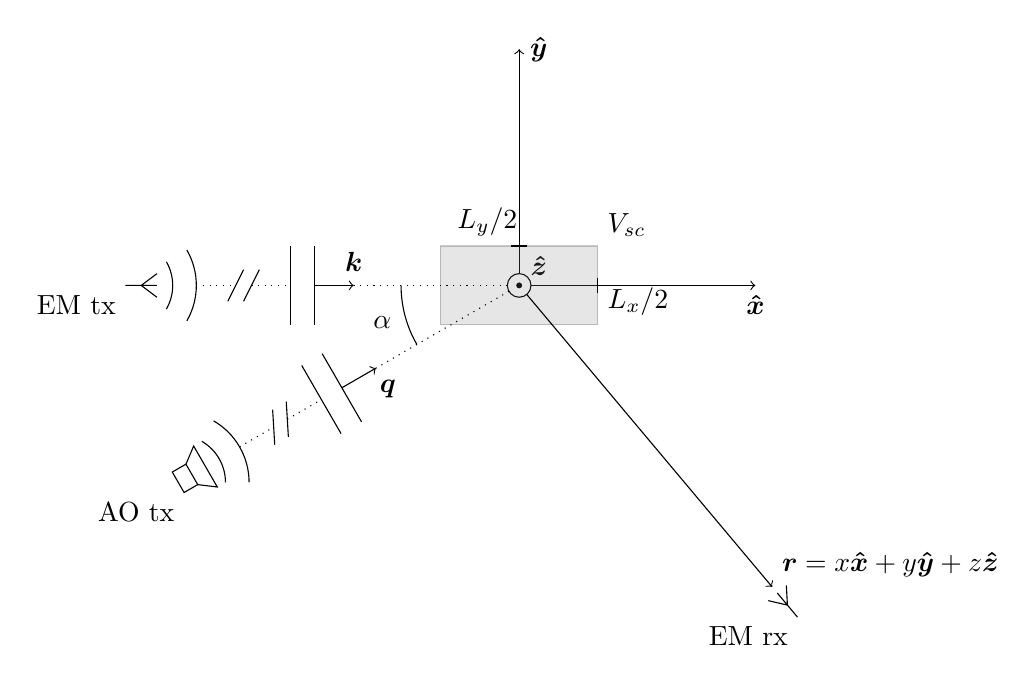
\begin{tikzpicture}
			% Draw coordinate axes
			\draw (0,0) circle(0.15);
			\filldraw[black] circle(0.03);
			\draw[->] (0.15,0) -- (3,0);
			\draw[->] (0,.150) -- (0,3);
			\draw (3,-0.25) node{$\bm{\hat{x}}$} (0.25,3) node{$\bm{\hat{y}}$} (0.25,0.25) node{$\bm{\hat{z}}$};
			
			% Draw scattering cube (or rectangle in this case)
			\draw[fill=gray,opacity=0.2] (-1,-0.5) rectangle(1,0.5);
			\draw (1,-0.1) -- (1,0.1) node[anchor= north west]{$L_x/2$} (-0.1,0.5) -- (0.1,0.5) node[anchor= south east]{$L_y/2$} (1,0.5) node[anchor=south west]{$V_{sc}$};
			
			% Draw EM tx and spherical waves
			\draw[shift = {(-5,0)}] (0,0) node[anchor=north east]{EM tx} -- (0.4,0) (0.2,0) -- (0.4,0.15)
			(0.2,0) -- (0.4,-0.15);
			\draw[shift = {(-5,0)}] ([shift={(-30:0.6)}] 0,0) arc(-30:30:0.6) ([shift={(-30:0.9)}] 0,0) arc(-30:30:0.9);
			
			% Draw EM "long distance" lines
			\draw[shift = {(-4.1,0)},dotted] (0,0) -- (0.5,0) (0.7,0) -- (1.2,0);
			\draw[shift = {(-4.1,0)}] (0.4,-0.2) -- (0.6,0.2) (0.6,-0.2) -- (0.8,0.2);
			
			% Draw EM plane waves
			\draw[shift = {(-2.9,0)}] (0,-0.5) -- (0,0.5) (0.3,-0.5) -- (0.3,0.5);
			\draw[shift = {(-2.6,0)}, ->] (0,0) -- (0.5,0);
			\draw[shift = {(-2.6,0)}] (0.5,0.3) node{$\bm{k}$};
			\draw[dotted] (-0.15,0) -- (-2.1,0);
			
			% Draw AO tx and spherical waves
			\draw[shift = {(210:5)}, rotate = 30] (0,-0.15) node[anchor=north east]{AO tx} rectangle (0.2,0.15) -- (0.4,0.3) -- (0.4,-0.3) -- (0.2,-0.15);
			\draw[shift = {(210:5)}, rotate = 30] ([shift={(-30:0.6)}] 0,0) arc(-30:30:0.6) ([shift={(-30:0.9)}] 0,0) arc(-30:30:0.9);
			
			% Draw AO "long distance" lines
			\draw[shift = {(210:4.1)}, rotate = 30,dotted] (0,0) -- (0.5,0) (0.7,0) -- (1.2,0);
			\draw[shift = {(210:4.1)}, rotate = 30] (0.4,-0.2) -- (0.6,0.2) (0.6,-0.2) -- (0.8,0.2);
			
			% Draw AO plane waves
			\draw[shift = {(210:2.9)}, rotate = 30] (0,-0.5) -- (0,0.5) (0.3,-0.5) -- (0.3,0.5);
			\draw[shift = {(210:2.6)}, rotate = 30, ->] (0,0) -- (0.5,0);
			\draw[shift = {(210:2.6)}, rotate = 30] (0.5,-0.3) node{$\bm{q}$};
			\draw[rotate = 30, dotted] (-0.15,0) -- (-2.1,0);
			
			% Draw angle alpha
			\draw ([shift={(180:1.5)}] 0,0) arc(180:210:1.5) (195:1.8) node{$\alpha$};
			
			% Draw line towards receiver
			\draw[->] (310:0.15) -- (310:5) node[anchor=south west]{$\bm{r} = x\bm{\hat{x}} + y\bm{\hat{y}} + z\bm{\hat{z}}$};
			
			% Draw EM rx
			\draw[shift = {(310:5.5)}, rotate = 130] (0,0) node[anchor=north east]{EM rx} -- (0.4,0) (0.2,0) -- (0.4,0.15) (0.2,0) -- (0.4,-0.15);
		\end{tikzpicture}
		\caption{\label{fig:radareq-geom} Geometry for the scattering problem.}
	\end{figure}
	The $xy$-plane is defined as the plane formed by the acoustic and electromagnetic wavevectors (they are assumed to be non-parallel). The scattering volume is centered in the origin of the coordinate system, and both the acoustic and electromagnetic waves are approximated as plane waves close to the origin. Thus, the electromagnetic and dielectric perturbation fields near the origin are defined as
	\begin{align*}
		\bm{E}_i (\bm{r}',t) &= \bm{E}_i (\bm{r}') = \bm{E}_{i0} e^{i\bm{k}\cdot\bm{r}'} \\
		\varepsilon_1 (\bm{r}',t) &= -\mathfrak{p} \varepsilon_r^2 S_0 \cos(\bm{q} \cdot \bm{r}' - \Omega t)
	\end{align*}
	Here, $\bm{E}_{i0}$ is the complex field amplitude at the origin ($-i\omega t$ time-dependence separated) and $\bm{k}$ is the electromagnetic wavevector. A scalar photoelastic relation has been assumed, where $\mathfrak{p}$ is the photoelastic constant, $S_0$ is the acoustic strain amplitude at the origin, $\bm{q}$ is the acoustic wavevector and $\Omega$ the acoustic frequency.
	
	For simplicity, the electromagnetic polarization is assumed to be perpendicular to the acoustic propagation direction, $\bm{E}_{i0} \cdot \bm{\hat{q}} = 0$. This is done to avoid polarization changes in the scattered field \cite{Korpel1988}. Due to this $\nabla(\bm{E}_i \cdot \nabla \varepsilon_1) = \bm{0}$ which simplifies the scattering integral to
	\begin{equation*}
		\bm{E}_{sc}(\bm{r},t) = \frac{k^2}{4\pi\varepsilon_r} \int_{V_{sc}} \frac{e^{ik |\bm{r}-\bm{r'}| }}{ |\bm{r}-\bm{r'}|} \bm{E}_i (\bm{r'},t) \varepsilon_1 (\bm{r'},t) \mathrm{d}v'
	\end{equation*}
	Insertion of the field expressions gives
	\begin{equation*}
	\bm{E}_{sc}(\bm{r},t) = -\frac{k^2}{4\pi\varepsilon_r} \int_{V_{sc}} \frac{e^{ik |\bm{r}-\bm{r'}| }}{ |\bm{r}-\bm{r'}|} \bm{E}_{i0} e^{i\bm{k} \cdot \bm{r}'} \mathfrak{p} \varepsilon_r^2 S_0 \cos(\bm{q} \cdot \bm{r}' - \Omega t) \mathrm{d}v'
	\end{equation*}
	Assuming far-field gives an approximation for the Green-function as \cite{Kristensson2008}
	\begin{equation*}
		\frac{e^{ik |\bm{r}-\bm{r'}| }}{ |\bm{r}-\bm{r'}|} \approx \frac{e^{ikr}}{r} e^{-ik \bm{\hat{r}} \cdot \bm{r}'}
	\end{equation*}
	where $r = |\bm{r}|$ and $\bm{\hat{r}} = \bm{r}/r$. The scattering integral is now written as
	\begin{equation*}
	\bm{E}_{sc}(\bm{r},t) = -\frac{\varepsilon_rk^2 e^{ikr}}{4\pi r} \bm{E}_{i0} \mathfrak{p} S_0 \int_{V_{sc}} e^{ik ( \bm{\hat{k}} - \bm{\hat{r}} ) \cdot \bm{r}'} \cos(\bm{q} \cdot \bm{r}' - \Omega t) \mathrm{d}v'
	\end{equation*}
	The cosine is now written as complex exponentials giving
	\begin{equation*}
		\bm{E}_{sc}(\bm{r},t) = -\frac{\varepsilon_rk^2 e^{ikr}}{8\pi r} \bm{E}_{i0} \mathfrak{p} S_0 \left( e^{-i\Omega t} \int_{V_{sc}} e^{i( k(\bm{\hat{k}} - \bm{\hat{r}}) + \bm{q} ) \cdot \bm{r}'} \mathrm{d}v + e^{i\Omega t} \int_{V_{sc}} e^{i( k(\bm{\hat{k}} - \bm{\hat{r}}) - \bm{q} ) \cdot \bm{r}'} \mathrm{d}v' \right)
	\end{equation*}
	The two integrals are of the same form, $\int e^{i\bm{A} \cdot \bm{r}'} \mathrm{d}v'$, where $\bm{A}$ is independent of $\bm{r}'$. This is solved in general below for the cuboid volume defined by $-L_m/2 \leq m \leq L_m/2$, $m = x,y,z$.
	\begin{multline*}
		\int_{V_{sc}} e^{i\bm{A} \cdot \bm{r}'} \mathrm{d}v' =
		\int_{V_{sc}} e^{i\bm{A} \cdot \bm{\hat{x}} x'} e^{i\bm{A} \cdot \bm{\hat{y}} y'} e^{i\bm{A} \cdot \bm{\hat{z}} z'} \mathrm{d}v' =
		\prod_{m = x,y,z} \frac{1}{i \bm{A} \cdot \bm{\hat{m}}} \left( e^{i\bm{A} \cdot \bm{\hat{m}} L_m/2} - e^{-i\bm{A} \cdot \bm{\hat{m}} L_m/2} \right) \\
		= \prod_{m = x,y,z} \frac{2}{\bm{A} \cdot \bm{\hat{m}}} \sin \left(\bm{A} \cdot \bm{\hat{m}} \frac{L_m}{2} \right) =
		\prod_{m = x,y,z} L_m \text{sinc} \left( \frac{\bm{A} \cdot \bm{\hat{m}} L_m}{2\pi} \right)
	\end{multline*}
	where sinc$(x) = \sin(\pi x)/(\pi x)$. To apply this result to $\bm{A} = k(\bm{\hat{k}} - \bm{\hat{r}}) \pm \bm{q}$ this is first simplified using the geometry defined earlier.
	\begin{equation*}
		k(\bm{\hat{k}} - \bm{\hat{r}}) \pm \bm{q} = k\bm{\hat{x}} - k(\bm{\hat{x}} x + \bm{\hat{y}} y + \bm{\hat{z}} z)/r \pm q(\bm{\hat{x}} \cos{\alpha} + \bm{\hat{x}} \sin{\alpha})
	\end{equation*}
	where r is not written out fully. The solution to the integral with this choice of $\bm{A}$ is now written as
	\begin{multline*}
		\int_{V_{sc}} e^{i(	k(\bm{\hat{k}} - \bm{\hat{r}}) \pm \bm{q}) \cdot \bm{r}'} \mathrm{d}v' =
		L_x \text{sinc} \left( \frac{L_x}{2\pi} ( k - kx/r \pm q\cos{\alpha} ) \right) \cdot
		L_y \text{sinc} \left( \frac{L_y}{2\pi} ( - ky/r \pm q\sin{\alpha} ) \right) \\
		\cdot L_z \text{sinc} \left( -\frac{L_z}{2\pi} kz/r \right)
	\end{multline*}
	Changing to spherical coordinates gives:
	\begin{multline*}
	\int_{V_{sc}} e^{i(	k(\bm{\hat{k}} - \bm{\hat{r}}) \pm \bm{q}) \cdot \bm{r}'} \mathrm{d}v' =
	L_x \text{sinc} \left( \frac{L_x}{2\pi} ( k - k\sin{\theta}\cos{\phi} \pm q\cos{\alpha} ) \right) \\
	\cdot L_y \text{sinc} \left( \frac{L_y}{2\pi} ( - k\sin{\theta}\sin{\phi} \pm q\sin{\alpha} ) \right)
	\cdot L_z \text{sinc} \left( -\frac{L_z}{2\pi} k\cos{\theta} \right) = L_x L_y L_z \Phi^\pm (\theta,\phi)
	\end{multline*}
	where all angular dependence has been gathered in the function $\Phi^\pm (\theta,\phi)$. This result is now inserted into the scattered field, giving
	\begin{equation*}
		\bm{E}_{sc}(\bm{r},t) = -\bm{E}_{i0} \frac{\varepsilon_rk^2 e^{ikr}}{8\pi r} \mathfrak{p} S_0 L_x L_y L_z \left( e^{-i\Omega t} \Phi^+ (\theta,\phi)  + e^{i\Omega t} \Phi^- (\theta,\phi) \right) = -\bm{E}_{i0} E_A(\bm{r},t)
	\end{equation*}
	
	By inspecting $E_A(\bm{r},t)$ it is clear that two frequency-shifted components arise. Since the implied time-dependence is $e^{-i\omega t}$, the factors $e^{\mp i\Omega t}$ give a frequency shift of $\pm \Omega$. The scattered field is written using two distinct components as
	\begin{equation*}
		\bm{E}_{sc} (\bm{r},t) = -\bm{E}_{i0} \left( E_A^+ (\bm{r},t) + E_A^- (\bm{r},t) \right)
	\end{equation*}
	where
	\begin{equation*}
		E_A^\pm (\bm{r},t) = \frac{\varepsilon_rk^2 e^{ikr}}{8\pi r} \mathfrak{p} S_0 L_x L_y L_z e^{\mp i\Omega t} \Phi^\pm (\theta,\phi)
	\end{equation*}
	
	\subsubsection{Solution in terms of power}
	This treatment has primarily been focused around the electric field. To obtain a more practical expression, this is not transformed into power. The scattered power density is given by
	\begin{equation*}
		\bm{S}_{sc} = \frac{1}{2} \bm{E}_{sc} \times \bm{H}_{sc}^*
	\end{equation*}
	with the magnetic field $\bm{H}_{sc}$ given by
	\begin{equation*}
		\bm{H}_{sc} \approx \frac{1}{ik \eta_0 \eta} \nabla \times \bm{E}_{sc}
	\end{equation*}
	where $\eta_0$ is the wave impedance of free space and $\eta_0 \eta$ the wave impedance in the material. An approximation has been made for $k$, where this is assumed to have the same value as before scattering. Since there is a frequency shift this is known to not be the case, but given a small acoustic frequency compared to the electromagnetic frequency, the error is small. The rotation of $\bm{E}_{sc}$ is now written as
	\begin{equation*}
		\nabla \times \bm{E}_{sc} = -\nabla \times (\bm{E}_{i0} E_A (\bm{r},t)) = -\nabla E_A (\bm{r},t) \times \bm{E}_{i0}
	\end{equation*}
	In spherical coordinates the gradient is written
	\begin{equation*}
		\nabla E_A = \frac{\partial E_A}{\partial r} \bm{\hat{r}} + \frac{1}{r} \frac{\partial E_A}{\partial \theta} \bm{\hat{\theta}} + \frac{1}{r\sin{\theta}} \frac{\partial E_A}{\partial \phi} \bm{\hat{\phi}}
	\end{equation*}
	$E_A$ contains a factor $1/r$, so the two last terms in the gradient will be $\sim 1/r^2$ and are neglected. The gradient is now written as
	\begin{equation*}
		\nabla E_A \approx \frac{\partial E_A}{\partial r} \bm{\hat{r}} = \left( \frac{ike^{ikr}}{r} - \frac{e^{ikr}}{r^2} \right) \frac{\varepsilon_r k^2}{8\pi} \mathfrak{p} S_0 L_x L_y L_z \left( e^{- i\Omega t} \Phi^+ (\theta,\phi) + e^{ i\Omega t} \Phi^- (\theta,\phi) \right) \bm{\hat{r}} \approx ikE_A \bm{\hat{r}}
	\end{equation*}
	where the $1/r^2$ term was neglected. These results are inserted into the expression for the magnetic field, giving
	\begin{equation*}
		\bm{H}_{sc} = \frac{1}{ik \eta_0 \eta} (-ikE_A \bm{\hat{r}} \times \bm{E}_{i0}) = \frac{E_A}{ \eta_0 \eta} \bm{\hat{r}} \times \bm{E}_{i0}
	\end{equation*}
	Now, the power density is written as
	\begin{equation*}
		\bm{S}_{sc} = \frac{1}{2} E_A \bm{E}_{i0} \times \left( \frac{E_A}{ \eta_0 \eta} \bm{\hat{r}} \times \bm{E}_{i0} \right)^* = \frac{|E_A|^2}{2\eta_0 \eta} \left( \bm{\hat{r}} (\bm{E}_{i0} \cdot \bm{E}_{i0}^*) - \bm{E}_{i0}^* (\bm{E}_{i0} \cdot \bm{\hat{r}}) \right)
	\end{equation*}
	In the far-field $\bm{E}_{sc} \cdot \bm{\hat{r}} = 0$ and since $\bm{E}_{sc} \parallel \bm{E}_{i0}$ the power density is simplified to
	\begin{equation*}
	\bm{S}_{sc} = \frac{\bm{\hat{r}}}{2\eta_0 \eta} |\bm{E}_{i0}|^2 |E_A (\bm{r},t)|^2
	\end{equation*}
	Since there is an implied $e^{-\omega t}$ time-dependence, this is added back in to obtain a time-average on the short time-scale ($\omega$ and not $\Omega$). This is
	\begin{equation*}
		\left< \bm{S}_{sc} e^{-i\omega t} \right> = \mathrm{Re}\left\{ \bm{S}_{sc} e^{-i\omega t} \right\} = \frac{\bm{\hat{r}}}{2\eta_0 \eta} |\bm{E}_{i0}|^2 |E_A (\bm{r},t)|^2
	\end{equation*}
	If the two frequency components are now considered individually,
	\begin{equation*}
		|E_A^\pm (\bm{r},t)|^2 =\frac{\varepsilon_r^2 k^4}{64 \pi^2 r^2} \mathfrak{p}^2 S_0^2 L_x^2 L_y^2 L_z^2 \Phi^\pm (\theta,\phi)^2
	\end{equation*}
	
	To find an expression for $|\bm{E}_{i0}|^2$, the field from the transmitter antenna is written as (adapted from \cite{Orfanidis2016})
	\begin{equation*}
		\bm{E}_T (\bm{r}) = ik\eta_0\eta \frac{e^{ikr}}{4\pi r} \bm{F}_\perp (\bm{\hat{r}})
	\end{equation*}
	where $\bm{F}_\perp$ is the far-field amplitude. Now the coordinate system is not the same as earlier in the derivation! Here it is a spherical coordinate system with origin at the transmitting antenna. This corresponds to a translation in $-\bm{\hat{x}}$ of the original coordinate system. Let $R_T$ be the distance between the two coordinate systems, or equivalently the distance from the transmitter to the scattering center. The direction to the scattering center in this new system is denoted $\bm{\hat{r}}_{sc} = \bm{r}_{sc}/R_T$. Assuming that the orientations of the transmitter and scattering coordinate systems are the same, $|\bm{E}_{i0}|^2$ can be written in the transmitter system as \cite{Orfanidis2016}
	\begin{equation*}
		|\bm{E}_{i0}|^2 = |\bm{E}_T(\bm{r}_{sc})|^2 = \left| ik\eta_0\eta \frac{e^{ikR_T}}{4\pi R_T} \bm{F}_\perp (\bm{\hat{r}}_{sc}) \right|^2 = \frac{k^2 \eta_0^2 \eta^2}{16 \pi^2 R_T^2} |\bm{F}_\perp (\bm{\hat{r}}_{sc})|^2 = 2\eta_0 \eta \mathcal{P}(\bm{\hat{r}}_{sc})
	\end{equation*}
	If the maximum gain $G_T$ of the antenna is in the direction $\hat{r}_{sc}$, it holds that \cite{Orfanidis2016}
	\begin{equation*}
		\mathcal{P}(\bm{\hat{r}}_{sc}) = \frac{P_T G_T}{4\pi R_T^2}
	\end{equation*}
	where $P_T$ is the power accepted by the antenna. This is used to write
	\begin{equation*}
		|\bm{E}_{i0}|^2 = 2\eta_0 \eta \frac{P_T G_T}{4\pi R_T^2}
	\end{equation*}
	Now this is inserted into the time-average of the power density
	\begin{equation*}
		\left< \bm{S}_{sc} e^{-i\omega t} \right>^\pm = \bm{\hat{r}} \frac{P_T G_T}{4\pi R_T^2} \frac{\varepsilon_r^2 k^4}{64 \pi^2 r^2} \mathfrak{p}^2 S_0^2 L_x^2 L_y^2 L_z^2 \Phi^\pm (\theta,\phi)^2
	\end{equation*}
	
	Now the effects of the receiving antenna are considered. It is assumed that this antenna is optimally directed towards the scattering center. The received power is then
	\begin{equation*}
		P_R^\pm = \left| \left< \bm{S}_{sc} e^{-i\omega t} \right>^\pm \right| A_e
	\end{equation*}
	where $A_e$ is the effective area of the antenna, which can be rewritten as
	\begin{equation*}
		A_e = \frac{\lambda_R^2 G_R}{4\pi}
	\end{equation*}
	where $G_R$ is the gain of the receiving antenna. $\lambda_R$ should be the wavelength at the antenna here, which is not necessarily the same as in the material. Combining this with earlier results gives a received power of
	\begin{equation*}
		P_R^\pm = \frac{\lambda_R^2 G_R}{4\pi} \frac{P_T G_T}{4\pi R_T^2} \frac{\varepsilon_r^2 k^4}{64 \pi^2 R_R^2} \mathfrak{p}^2 S_0^2 L_x^2 L_y^2 L_z^2 \Phi^\pm (\theta,\phi)^2
	\end{equation*}
	where $R_R$ is the distance between the scattering center and the receiver, and the receiver is located in the direction $(\theta,\phi)$ as seen from the scattering center. For a more traditional bistatic radar equation this can be written as
	\begin{equation*}
	P_R^\pm = \frac{P_T R_T G_R \lambda_R^2 \sigma^\pm (\theta,\phi)}{(4\pi)^3 R_T^2 R_R^2}
	\end{equation*}
	with the radar cross-section given by
	\begin{equation*}
		\sigma^\pm (\theta, \phi) = \frac{\varepsilon_r^2 k^4}{16\pi} \mathfrak{p}^2 S_0^2 L_x^2 L_y^2 L_z^2 \Phi^\pm (\theta,\pi)^2
	\end{equation*}
	
	\subsubsection{Signal-to-noise ratio and coherent integration}
	A more practical measurement than received power is signal-to-noise ratio (SNR). For this, the average noise power is described as \cite{Young2004}
	\begin{equation*}
		P_n = kTB
	\end{equation*}
	where $k$ is Boltzmann's constant, $T$ is the temperature and $B$ is the utilized receiver bandwidth. The noise power picked up by the antenna is calculated using the standard temperature $T_0 = 290$ K. The SNR directly at the antenna can thus be written as
	\begin{equation*}
		\mathit{SNR}^\pm_{ant} \frac{P_T R_T G_R \lambda_R^2 \sigma^\pm (\theta,\phi)}{(4\pi)^3 R_T^2 R_R^2 kT_0 B}
	\end{equation*}
	After the antenna is the RF front-end which usually contains a bandpass filter, low-noise amplifier (LNA), and mixer. Here the received signal is amplified so that it can be further processed. The amplification affects both the signal and noise, but the electronic components add more noise which causes the SNR to deteriorate. To quantify this, the concept of noise ratio and noise figure is used. The noise ratio is defined as \cite{Young2004}
	\begin{equation*}
		\mathit{NR} = \frac{\mathit{SNR}_i}{\mathit{SNR}_o}
	\end{equation*}
	where the SNR's are in linear units, $i$ denotes input and $o$ denotes output. It is more common to use noise figure, which is simply the noise ratio expressed in dB units, $\mathit{NF} = 10\log_{10}(\mathit{NR})$. Most of the noise is added at the RF front-end, so it is usually sufficient to use a noise ratio/figure for that part of the receiver. The SNR after the receiver can now be written using the noise ratio as
	\begin{equation*}
		\mathit{SNR}^\pm = \frac{P_T R_T G_R \lambda_R^2 \sigma^\pm (\theta,\phi)}{(4\pi)^3 R_T^2 R_R^2 kT_0 B \cdot \mathit{NR}}
	\end{equation*}
	One more effect is added to this, and that is signal integration in the signal processing following the receiver. Noise can often be modeled as a random process, and if multiple samples are added together the noise can be averaged out. If coherent demodulation is used, $N$ samples added together will cause the SNR to improve by a factor $N$ \cite{Richards2012}. The SNR can then be written as
	\begin{equation*}
		\textit{SNR}^\pm_N = \frac{P_T R_T G_R \lambda_R^2 \sigma^\pm (\theta,\phi)}{(4\pi)^3 R_T^2 R_R^2 kT_0 B \cdot \mathit{NR}} N
	\end{equation*}
	
	\subsection{Geometry for maximum scattering \label{app:braggmax}}
	Let us begin with the $\Phi$ angular dependence function:
	\begin{multline*}
	\Phi^\pm(\theta,\phi) = \text{sinc} \left( \frac{L_x}{2\pi} \left( k - k\sin{\theta}\cos{\phi} \pm q\cos{\alpha} \right) \right) 
	\cdot \text{sinc} \left( \frac{L_y}{2\pi} \left( -k\sin{\theta}\sin{\phi} \pm q\sin{\alpha} \right) \right) \\
	\cdot \text{sinc} \left( -\frac{L_z}{2\pi} k\cos{\theta} \right)
	\end{multline*}
	The maximum of this function mush be where all sinc-functions are maximum. For a sinc the maximum is given when the argument is equal to 0, which simplifies the process. Firstly, consider the third sinc:
	\begin{equation*}
		\text{sinc} \left( -\frac{L_z}{2\pi} k\cos{\theta} \right)
	\end{equation*}
	The argument of this is obviously zero when $\cos{\theta} = 0$, which for $0 \leq \theta \leq \pi$ is when $\theta = \pi/2$. This fixes the maximum to the plane formed by the incident electromagnetic and acoustic wavevectors. What it means is that the scattering occurs primarily in one single interaction plane, which simplifies analysis. Now the arguments of the two other sinc functions are set to zero with the value for $\theta$ being set to $\pi/2$:
	\begin{align}
		k - k\cos{\phi} \pm q\cos{\alpha} &= 0 \label{eq:bragg-sinc1} \\
		-k\sin{\phi} \pm q\sin{\alpha} &= 0 \label{eq:bragg-sinc2}
	\end{align}
	This system of equations is now used to find the direction of the maximum. TO avoid confusion, the positive and negative versions of the system are considered separately.
	
	\subsubsection{(+) case}
	Begin with equation \ref{eq:bragg-sinc1}:
	\begin{equation*}
		\cos{\alpha} = \frac{k}{q}\left( \cos{\phi} - 1 \right) = \frac{k}{q}\left( \pm \sqrt{1-\sin^2{\phi}} - 1 \right)
	\end{equation*}
	Now equation \ref{eq:bragg-sinc2} is inserted in the above as
	\begin{equation*}
		\cos{\alpha} = \frac{k}{q}\left( \pm \sqrt{1-\frac{q^2}{k^2}\sin^2{\alpha}} - 1 \right)
	\end{equation*}
	This is rewritten as
	\begin{equation*}
		\pm \sqrt{k^2-q^2\sin^2{\alpha}} = q\cos{\alpha} + k
	\end{equation*}
	And squared
	\begin{equation*}
		k^2 - q^2\sin^2{\alpha} = q^2\cos^2{\alpha} + 2kq\cos{\alpha} + k^2
	\end{equation*}
	After some simplification, the following equation is obtained:
	\begin{equation*}
		\cos{\alpha} = -\frac{q}{2k}
	\end{equation*}
	This is now inserted in equation \ref{eq:bragg-sinc1} and \ref{eq:bragg-sinc2}:
	\begin{align*}
		k - k\cos{\phi} - \frac{q^2}{2k} &= 0 \\
		-k\sin{\phi} \pm q\sqrt{1-\frac{q^2}{4k^2}} &= 0
	\end{align*}
	Rearranging gives
	\begin{align*}
		\cos{\phi} &= 1 - \frac{q^2}{2k^2} \\
		\sin{\phi} &= \pm \frac{q}{k} \sqrt{1-\frac{q^2}{4k^2}}
	\end{align*}
	The second equation can be further constrained by utilizing $0 \leq \alpha \leq \pi$. This gives $\sin{\alpha} \geq 0$. With $k,q \geq 0$ and equation \ref{eq:bragg-sinc2}: $\sin{\phi} = \frac{q}{k}\sin{\alpha} \geq 0$. Thus, the only valid solution is the positive one. Now, the cos and sin equations are combined into a tan equation:
	\begin{equation*}
		\tan{\frac{\phi}{2}} = \frac{1 - \cos{\phi}}{\sin{\phi}} = \frac{1 - \left( 1 - \frac{q^2}{2k^2} \right)}{\frac{q}{k} \sqrt{1-\frac{q^2}{4k^2}}} = \frac{\frac{q^2}{2k^2} }{\frac{q}{k} \sqrt{1-\frac{q^2}{4k^2}}} = \frac{q}{2k\sqrt{1-\frac{q^2}{4k^2}}} = \sqrt{\frac{q^2}{4k^2-q^2}}
	\end{equation*}
	
	\subsubsection{(-) case}
	This case is the same as the (+) case, but with some sign changes. Begin with equation \ref{eq:bragg-sinc1}:
	\begin{equation*}
	\cos{\alpha} = \frac{k}{q}\left( 1 - \cos{\phi} \right) = \frac{k}{q}\left( 1 \pm \sqrt{1-\sin^2{\phi}} \right)
	\end{equation*}
	Now equation \ref{eq:bragg-sinc2} is inserted in the above as
	\begin{equation*}
	\cos{\alpha} = \frac{k}{q}\left( 1 \pm \sqrt{1-\frac{q^2}{k^2}\sin^2{\alpha}} \right)
	\end{equation*}
	This is rewritten as
	\begin{equation*}
	\pm \sqrt{k^2-q^2\sin^2{\alpha}} = q\cos{\alpha} - k
	\end{equation*}
	And squared
	\begin{equation*}
	k^2 - q^2\sin^2{\alpha} = q^2\cos^2{\alpha} - 2kq\cos{\alpha} + k^2
	\end{equation*}
	After some simplification, the following equation is obtained:
	\begin{equation*}
	\cos{\alpha} = \frac{q}{2k}
	\end{equation*}
	This is now inserted in equation \ref{eq:bragg-sinc1} and \ref{eq:bragg-sinc2}:
	\begin{align*}
	k - k\cos{\phi} - \frac{q^2}{2k} &= 0 \\
	-k\sin{\phi} \pm q\sqrt{1-\frac{q^2}{4k^2}} &= 0
	\end{align*}
	Rearranging gives
	\begin{align*}
	\cos{\phi} &= 1 - \frac{q^2}{2k^2} \\
	\sin{\phi} &= \pm \frac{q}{k} \sqrt{1-\frac{q^2}{4k^2}}
	\end{align*}
	The second equation can be further constrained by utilizing $0 \leq \alpha \leq \pi$. This gives $\sin{\alpha} \geq 0$. With $k,q \geq 0$ and equation \ref{eq:bragg-sinc2}: $\sin{\phi} = -\frac{q}{k}\sin{\alpha} \leq 0$. Thus, the only valid solution is the negative one. Now, the cos and sin equations are combined into a tan equation:
	\begin{equation*}
	\tan{\frac{\phi}{2}} = \frac{1 - \cos{\phi}}{\sin{\phi}} = \frac{1 - \left( 1 - \frac{q^2}{2k^2} \right)}{-\frac{q}{k} \sqrt{1-\frac{q^2}{4k^2}}} = -\sqrt{\frac{q^2}{4k^2-q^2}}
	\end{equation*}
	
	\subsubsection{Summary}
	The equations for both the (+) and (-) case are very similar, and can be written in a simple way using $\pm$ signs. The conditions define the geometry which gives the maximum scattering through the angle $\alpha$ between EM and acoustic incident waves and the angles $\theta$ and $\phi$ for the receiver direction. They are summarized below:
	\begin{align}
			\theta &= \pi/2 \label{eq:bragg-theta}\\
			\cos{\alpha} = \mp \frac{q}{2k} &= \mp \frac{\lambda}{2\Lambda} \label{eq:bragg-alpha}\\
			\tan{\frac{\phi}{2}} = \pm \sqrt{\frac{q^2}{4k^2-q^2}} &= \pm \sqrt{\frac{\lambda^2}{4\Lambda^2-\lambda^2}} \label{eq:bragg-phi}
	\end{align}
	
	In acousto-optics the interaction occurs in a single plane, which is what (\ref{eq:bragg-theta}) describes. There is also a Bragg condition defining the angle between an acoustic and optic wave which is required for maximum reflection. This is presented in \cite{Saleh2007} as
	\begin{equation*}
		\sin{\theta_B} = \frac{\lambda}{2\Lambda}
	\end{equation*}
	where $\theta_B$ relates to this geometry as $\alpha = \pi/2 \pm \theta_B$ (see figures 19.1-2 and 19.1-5 in \cite{Saleh2007}). Here, (\ref{eq:bragg-alpha}) is used to obtain the optimal angle between electromagnetic and acoustic waves, and the transformation between $\alpha$ and $\theta_B$ can be inserted as
	\begin{equation*}
		\cos{\alpha} = \cos(\pi/2 \pm \theta_B) = \mp \sin{\theta_B}
	\end{equation*}
	The RHS of (\ref{eq:bragg-alpha}) is $\mp \lambda/2\Lambda$. This should be equal to the RHS above, which directly gives the Bragg condition.
	
	In acousto-optics there is no separate equation for the scattering angle as in (\ref{eq:bragg-phi}) above. This is simply assumed to be the same as the incident angle, which gives $\phi = \pm 2\theta_B$ (again, see figures 19.1-2 and 19.1-5 in \cite{Saleh2007}). This is inserted, giving
	\begin{equation*}
		\tan{\frac{\phi}{2}} = \tan(\pm \theta_B) = \pm \frac{\sin{\theta_B}}{\cos{\theta_B}} = \pm \sqrt{\frac{\sin^2{\theta_B}}{1-\sin^2{\theta_B}}}
	\end{equation*}
	The RHS of (\ref{eq:bragg-phi}) is
	\begin{equation*}
		\pm \sqrt{\frac{\lambda^2}{4\Lambda^2-\lambda^2}} = \pm \sqrt{\frac{(\lambda/2/\Lambda)^2}{1-(\lambda/2\Lambda)^2}}
	\end{equation*}
	If this is compared with the RHS above, the Bragg condition is once again obtained.
	So, from simple variable substitutions the same results as in acousto-optics are obtained. This gives the model some validation since it is in agreement with an already established theory.
	
	\subsection{Drawing for spherical coordinates}
	\begin{figure}[H]
		\centering
		\tdplotsetmaincoords{60}{100}
		\begin{tikzpicture}[tdplot_main_coords,scale=5]
		% Draw cartesian coordinate axes
		\coordinate (0) at (0,0,0);
		\tdplotsetcoord{P}{1}{30}{45}
		\draw[->] (0) -- (1,0,0) node[anchor=north east]{$x$};
		\draw[->] (0) -- (0,1,0) node[anchor=north west]{$y$};
		\draw[->] (0) -- (0,0,1) node[anchor=south]{$z$};
		\tdplotdrawarc{(0)}{0.3}{0}{45}{anchor=north}{$\phi$}
		\tdplotsetthetaplanecoords{45}
		\tdplotdrawarc[tdplot_rotated_coords]{(0)}{0.3}{0}{30}{anchor=south}{$\theta$}
		\draw[dashed] (0) -- (Pxy) (0) -- (P) -- (Pxy) (P) node[anchor=south west]{$(r,\theta,\phi)$};
		\draw[shift = {(P)}] (0,-0.03,-0.03) -- (0,0.03,0.03) (0,0.03,-0.03) -- (0,-0.03,0.03);
		\end{tikzpicture}
		\caption{\label{fig:spherical-coords} Spherical coordinate system used.}
	\end{figure}
	
	\small
	\bibliographystyle{../../Litteratur/IEEEtran}
	\bibliography{../../Litteratur/litteratur}
	
\end{document}